% !TEX root = BusSim.tex
\section{Methodology\label{s:method}}

%\subsection{Notation}

%The following notation will be used to formalise each of the simulation models:
%\textbf{can the notation be put in the appendix as it takes up alot of room?}
%\label{s:Notation}
%\begin{itemize}
   % \item $dt$: Time interval ($s$)
    %\item $t$: Current time ($s$ from 00:00:00)
    %\item $N$: Number of buses
	%\item $j$: Index of vehicle $(j=1..N)$
%	\item $m$: Index of bus stop $(m=1..M)$
%	\item $M$: Number of bus stops
%	\item $c_j$: Current status of bus j (IDLE, MOVING, DWELLING or FINISHED). Where IDLE refers to out-of-service buses and DWELLING refers to buses that are serving passengers at stops. 
%	\item $a_j$: Acceleration rate of bus j ($m/s^2$)
%	\item $v_j$: Current speed of bus j ($m/s$)
%	\item $Occ_{j}$: Current occupancy of bus $j$ (number of passengers onboard)
%	\item $H$: Scheduled headway ($s$)
%	\item $C$: Bus capacity
%	\item $V$: Traffic speed ($m/s$)
%	\item $\delta_j$: The scheduled dispatch time of bus $j$ from the first stop
%	\item $t^a_{j,m}$: Arrival time of bus $j$ at stop $m$
%	\item $t^d_{j,m}$: The moment when bus $j$ can leave stop $m$ after passenger boarding and alighting (or $Leave\_stop\_time$)
   % \item $D_{j,m}$: Dwell time of bus $j$ at stop $m$ for passenger boarding and alighting
%	\item $\theta_1,\theta_2,\theta_3$: Parameters set for estimating $D_{j,m}$
%	\item $B_{j,m}$: Number of boarding passenger to bus $j$ at stop $m$
%	\item $A_{j,m}$: Number of alighting passenger from bus $j$ at stop $m$
%	\item $Arr_m$: Arrival rate of passengers to stop $m$ per second
%	\item $Dep_m$: Departure rate of passengers from stop $m$
%\end{itemize}

\subsection{A hypothetical version of reality: BusSim-truth and its two simpler variations}


The first step in the proposed workflow is to develop an agent-based bus route model that will be used to generate synthetic GPS data for each bus on the route (BusSim-truth). BusSim-truth is a stochastic and dynamic model with two classes of agents (bus and bus stop) and predefined parameters (see Table \ref{tab:Agents} ). It is stochastic because the number of boarding passengers is drawn from a random distribution, and dynamic because it parameters gradually change over time. The level of stochasticity and dynamicity in BusSim-truth can also be adjusted to represent bus route systems where conditions are largely stable or volatile over time.  

Figure \ref{fig:BusSim_flowchart} illustrates the workflow for BusSim-truth. Only a brief explanation of the model is included here, as more information on how the BusSim-truth model works can be found in the Appendix A. 
At each current time step, each Bus agent checks whether the next time step would be larger than the vehicle's scheduled dispatch time. If it is, we then check whether the bus is on the road (Status equals $MOVING$), or at a stop for passenger dwelling (Status equals $DWELLING$), or has finished its service (Status equals $FINISHED$), otherwise the bus remains $IDLE$.  

If the status is $MOVING$, we first check whether the bus is at a bus stop, by comparing the $GeoFence$ area of each bus stop agent with the bus' location. If the bus is not approaching a bus stop, its current speed will be compared with the surrounding traffic speed. In the case it is slower, we assume that the bus will speed up. If the speed already matches the traffic speed, the bus will maintain the same speed. Currently the traffic volume on the whole network is represented as a single dynamic parameter, although in practice it would be relatively trivial to make the traffic volume heterogeneous across the network. The system will first check if the stop is at the last stop when the bus is approaching a bus stop, where the bus' status will be changed to $FINISHED$ and the bus speed changed to zero. If it is not the last stop, the system will change the status of agent Bus to $DWELLING$ and its speed to zero. 
%Full details of how BusSim-truth works can be found in the Appendix.

\begin{table}[htbp]
  \centering
  \caption{Type of agents and their parameters in BusSim-truth}
    \resizebox{\textwidth}{!}{\begin{tabular}{ll}
    %\toprule
    \textbf{Parameter} & \textbf{Description} \\
    \midrule
     BusID  & Unique ID of the bus agent \\
          Acceleration & The acceleration value in $m/s^2$ if the bus needs to accelerate \\
           StoppingTime & Deadtime due to door opening and closing if the bus has to stop \\
           Visited & List of visited bus stops \\
           States & Whether the bus is idle, moving, dwelling or finished \\
           Trajectory & GPS coordinates of bus locations \\
    \midrule
    bus stopID & Unique ID of the bus stop \\
           Position & Distance from the first stop \\
           $Arr_m$ & Passengers arrived to the stop per second \\
           $Dep_m$ & Percentage of onboard passengers alight at the stop \\
           Arrival\_time & Store actual arrival time of buses at the stop \\
           GeoFence & A circle area to identify whether the bus is at the bus stop \\
    \bottomrule
    \end{tabular}}%
  \label{tab:Agents}%
\end{table}%

\begin{figure}[ht]
    \centering
    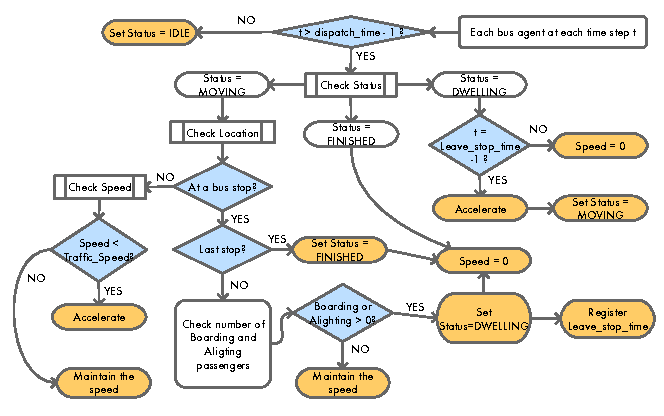
\includegraphics[width=1\textwidth]{Figures/flowchart.pdf}
    \caption{Flowchart of BusSim-truth.}
    \label{fig:BusSim_flowchart}
\end{figure}

As described in Section \ref{s:problem}, we use BusSim-truth to generate two sets of synthetic data: (1) `historical' GPS data that simulate normal bus route operation over a number of days and are used for calibration; and (2) `real-time' GPS data that represents a single run of the model and are used to represent the bus system \textit{today}. These are visualised in Figure~\ref{fig:historical_realtime}. Each record in the synthetic data is called an \textit{observation vector}. The vector contains all of the observations made from the `real world' (in this case the BusSim-truth).

\begin{figure}[h]
	\centering
	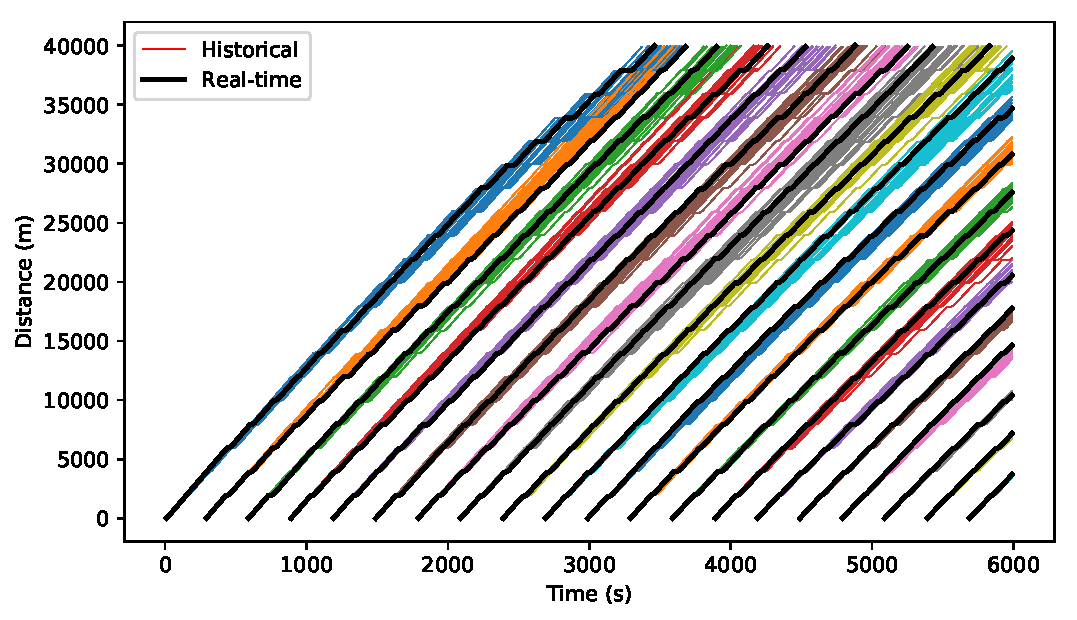
\includegraphics[width=1\textwidth]{Figures/Fig_spacetime_dynamic.pdf}
	\caption{Synthetic `historical' versus `real-time' GPS bus location data. Each coloured line shows the trajectory of one bus in the `historical' GPS data. As the BusSim-truth model is stochastic, there are differences between the trajectories. This is similar to the reality where buses operate slightly differently on multiple days. The bold black lines are another instance of bus trajectory that we consider as the `real-time' GPS data.  }
	\label{fig:historical_realtime}
\end{figure}

%\end{enumerate}

\subsection{Optimising the parameters of BusSim-deterministic and BusSim-stochastic}
\label{s:calibration}

Most agent-based models have a large number of parameters. For the BusSim models, the model parameter vector $S_t$ at time $t$ contains the arrival rate $Arr_m^t$, departure rate $Dep_m^t$ at each stop $m$, and the traffic speed $V^t$. 
\begin{equation}
  S_t  = \left[ \begin{array}{ccc}
Arr_m^t & Dep_m^t & V^t  
\end{array} \right] \quad m=1..M 
\label{eq:S}
\end{equation} 

The two simpler models (BusSim-deterministic and BusSim-stochastic) first need to be calibrated to the observations (the historical data). Here an automatic parameter calibration process, based on the Cross-Entropy Method (CEM) \citep{rubinstein1999cross} is used. CEM is a population-based Monte Carlo learning algorithm to combinatorial multi-extremal optimisation and importance sampling. It originated from the field of rare event simulation, where even small probabilities need to be estimated \citep{rubinstein1999cross}. In principle, CEM develops a \textit{probability distribution} over possible solutions for the optimal parameters of the model. New solution candidates are drawn from this distribution and are evaluated. The best candidates are then selected to form a new improved probability distribution of the optimal parameters, until certain criteria are met. CEM is chosen over some other popular optimisation methods in parameter calibration of ABMs, such as Genetic Algorithm \citep{heppenstall_genetic_2007} and simulated annealing~\citep{pennisi_optimal_2008}, because of its probabilistic nature that facilitates the calibration of stochastic models \citep{ngoduy2012calibration}. The interested reader may refer to \citep{rubinstein1999cross}, and various applications of CEM, such as \citep{ngoduy2012calibration}, for a more detailed account. A pseudo-code of the CEM algorithm that we adopted for this paper has also been described in Appendix B. 

Formally, the parameter calibration is an optimisation problem to minimise some performance index $PI(\pi)$ over all $\pi \in \mathbb{R}^k$. Here a solution $\pi= (\pi_1,\pi_2,...,\pi_k)$ denotes a set of parameters of the model under consideration and $k$ denotes the number of dimension in this set. Let $\pi_*$ denote the optimal solution, or the best set of model parameters that we want to find, that is:

\begin{equation}
    \pi_* = \text{argmin} \quad PI(\pi), \quad \pi \in \mathbb{R}^n
\end{equation}

The above objective function is equivalent to finding $\pi_*$ such that $PI(\pi_*) \leq PI(\pi) \quad \forall X \in \Pi$, where $\Pi$ is a constrained parameter space such that $\Pi \in \mathbb{R}^k$. The performance index $PI(\pi)$ is generally the difference between model output and observed data. The complexity of this problem comes from the stochasticity of BusSim, where the same solution $\pi$ may yield a different realisation $PI(\pi)$. To reduce this stochastic effect, it is necessary to run the (stochastic) model multiple times, and to evaluate the simulation outputs against a compilation of observed data from multiple days or instances. Let $K_I$ be the number of replications required for each model evaluation and $K_O$ be the number of instances in the observed data, we can derive a more detailed objective function of the parameter calibration problem: 

\begin{align}
    \text{min} \ PI(\pi) = \frac{1}{N \cdot T} \sum_{t=1}^T \sum_{n=1}^N \Bigg[ \bigg|  \frac{1}{K_I} \sum^{K_I}  s_{j,i,t}^{SIM}  - \frac{1}{K_O} \sum^{K_O}  s_{j,o,t}^{OBS} \bigg| + \nonumber \\
    \bigg| \sqrt{\frac{\sum^{K_I} \big( s_{j,i,t}^{SIM} - \hat{s}_{j,i,t}^{SIM} \big)^2}{K_I-1}}  - \sqrt{\frac{\sum^{K_O} \big( s_{j,o,t}^{OBS} - \hat{s}_{j,o,t}^{OBS} \big)^2}{K_O-1}} \bigg|   \Bigg]
    \label{eq:objective_function}
\end{align}

Where $N$ is the number of buses, $T$ is the number of time steps, $s_{j,i,t}^{SIM}$ is the location of simulated bus agent $j$ at time $t$ for the replication $i$, and similarly $s_{j,o,t}^{OBS}$ is the synthetic observed location of bus $j$ at time $t$ for the instance $o$. The objective function in Equation \ref{eq:objective_function} can be seen as the sum of the difference in mean location and standard deviation of locations at each time step for each bus and each replication/instance between simulated outputs and synthetic observed data. We want to evaluate the difference in not just the mean but also the standard deviation of bus locations because the system under study is stochastic, so it is not just the mean but also the spread of bus locations over multiple instances are important. 

\subsection{Data Assimilation using a Particle Filter (PF)}
\label{s:PF}

We can formulate an ABM as a state-space model $\dot{X}_t = f(X_{t}) + \epsilon_t$ and use data assimilation (DA) to dynamically optimise the model variables with up-to-date data to reduce uncertainty. The state-space model is represented by a state-space vector $X_t$ at time $t$, which contains all information of the current state of each agent in the model: 
\begin{align}
    X_t = \left[ O_t \quad S_t \right] \nonumber \\
    =\left[ \begin{array}{ccccccc}
c_j^t & s_j^t & v_j^t & Occ_j^t & Arr_m^t & Dep_m^t & V^t \end{array} \right] 
\label{eq:state_vector}
\end{align}
  
The state-space vector $X_t$ must contain all of the information that identifies the current state of the modelled system, allowing it to be projected forward to the next time step. Thus vector $X_t$ usually contains both the observation vector $O_t$ and the model parameters vector $S_t$ (Equation \ref{eq:S}) at time $t$. Note that $S_t$ has been calibrated in the previous section, but is still included in the state space vector $X_t$ to allow the model to be dynamically optimised with new data -- this is essential in dynamic situations where parameter values change over time. This approach is often referred to as dynamic calibration \citep{eicker2014calibration}.

Data Assimilation (DA) is a suite of methods to adjust the state of a running model using new data to better represent the current state of the system under study \citep{ward_dynamic_2016}. DA was born out of data scarcity, where observation data are sparse and insufficient to describe the system. Notwithstanding the proliferation of new data sources, insufficient data is still a major problem in research. The prediction of bus locations is a clear example where the number of future boarding and alighting passengers are unknown in real time. DA algorithms fill in the spatio-temporal gaps in the observed data by running a model forward in time until new observed data are available. This is typically called the \textit{predict} step in DA algorithms. After the predict step, DA has an estimate of the current system state and its uncertainty (which is often referred as the `prior' in Bayesian literature). The next step is typically called the \textit{update} step, where new observations and uncertainty are used to update the current state estimates. The result is referred to as the `posterior' in Bayesian literature, and should be the best guest of the system state from both the observations and model.

There are several DA algorithms in the literature, ranging from the simple Kalman Filter \citep{meinhold1983understanding} to more advanced extensions, including extended, ensemble and unscented Kalman Filter \citep{ward_dynamic_2016}. These algorithms generally aim to extend the original Kalman Filter by relaxing the assumption of linearity and introducing methods to work with non-linear models. However, they may not be the most suitable candidate to incorporate data into ABMs for two reasons. First, ABMs are driven by a large number of interacting agents with goals, history and behavioural rules. As a result, they lack an analytic structure, such as differential or difference equations, to facilitate the implementation of the Kalman Filter and its extensions where often the model Jacobian and covariance matrices need to be formulated \citep{wang_data_2015}. Second, although the assumption of linearity has been relaxed, these extensions assume that the noise in the model estimation is Gaussian. 

There is a flexible Bayesian filtering method that has been designed to work with non-linear, non-Gaussian models without analytical structure; this is the Particle Filter (PF). The key idea is to approximate a posterior distribution by a set of samples or particles, drawn from this distribution. Each particle is a concrete hypothesis of the true system state. The set of particles approximates the posterior distribution. PF is best described as a nonparametric Bayes filter because it develops the belief using a finite number of samples. 

Hypotheses of the system state at time $t$ is represented by a set $P_t$ of $N_P$ weighted random particles: 
\begin{equation} 
    P_t =  \{  \langle X_t^{\nint{i}}, w_t^{\nint{i}} \rangle \ | \ i=1,...,N_P \}
\label{eq:system_state_particle}
\end{equation}

where $X_t^{\nint{i}}$ is the state vector of the \textit{i}-th particle and $w_t^{\nint{i}}$ is the corresponding weight. Weights are non-zero, and sum over all weights is 1. The core idea of the PF is to update and maintain this set of particles given model outputs and observations. A PF recursively estimates the particle set $P_t$ based on the estimate $P_{t-1}$ at the previous time step, and the observation. The PF algorithm can be briefly described in three steps:
\begin{enumerate}
	
    \item \textbf{Predict:} Generate the next set of particles $\hat{P}_t$ from the previous set $P_{t-1}$. This represents the \textit{prior} distribution to describe how the system state evolves. 
    \item \textbf{Importance Weighting:} Compute the importance weight $w_t^{\nint{i}}$ for each particle in $P_t$. This is equivalent to the `Update' step in Kalman Filter, and will give us the \textit{posterior} distribution 
    \item \textbf{Resampling:} This step has no analogous step in Kalman Filter and its extensions. The resampling step creates a new set of particles from the current set. The likelihood to draw a particle is proportional to its weight. We adopt Sample Importance Resampling (SIR), a popular bootstrap systematic resampling in the PF literature \citep{wang_data_2015, carrassi_data_2018}. SIR has been developed to deal with \textit{particle deprivation}, which is the problem when particles converge to a single particle after several iterations due to one particle outperforming all others \citep{kong_sequential_1994}. This problem significantly reduces the area of state space covered by the particles in later iterations. 
\end{enumerate}
    Since resampling will generate particles using the existing pool of particles, it will not be able to produce particles where the prediction accuracy is better than the existing particle pool. This means that in \textit{classical} PF, the model parameter $S_t$ of both BusSim-deterministic and BusSim-stochastic will be unchanged over time. Because the  parameters change over time, we need to dynamically optimise $S_t$. This problem is solved in this paper by a simple and generic solution. We improve the quality of the particles by diversification similar to \citep{vadakkepat_improved_2006}, in a process also known as roughening, jittering, and diffusing \citep{pantrigo_combining_2005}. This is achieved by adding a random Gaussian white noise $\sigma$ with mean 0 and a predefined standard deviation, not to the whole state vector $X_t$, but to the model parameter $S_t$, to increase the probability of having particles that represent the current state of the underlying model. 
    
The PF is applied to BusSim-deterministic and BusSim-stochastic using up-to-date data from the synthetic `real-time' GPS data. 

